\documentclass[12pt]{article}

\usepackage{fullpage}
\usepackage{multicol,multirow}
\usepackage{tabularx}
\usepackage{ulem}
\usepackage[utf8]{inputenc}
\usepackage[russian]{babel}
\usepackage{listings}
\usepackage{hyperref}
\usepackage{graphicx}
\DeclareGraphicsExtensions{.png}


\begin{document}

\section*{Лабораторная работа №\,4 по курсу криптографии}

Выполнила студентка группы М8О-307Б \textit{Довженко Анастасия}.

\subsection*{Условие}
Подобрать такую эллиптическую кривую над конечным простым полем порядка p, порядок точки которой полным перебором находится за 10 минут на ПК. Упомянуть в отчёте какие алгоритмы и теоремы существуют для облегчения и ускорения решения задачи полного перебора.

\subsection*{Метод решения}
Я использовала каноническую форму эллиптической кривой:
$$ y^{2} = x^{3} + ax + b$$
Коэффициенты $a$ и $b$ были выбраны случайно. Модуль кривой $p$ подбирался вручную, пока подсчёт порядка точки не стал удовлетворять условию. Сначала я построила график для небольших $p$, чтобы посмотреть, как изменяется время. Вот что получилось:\\
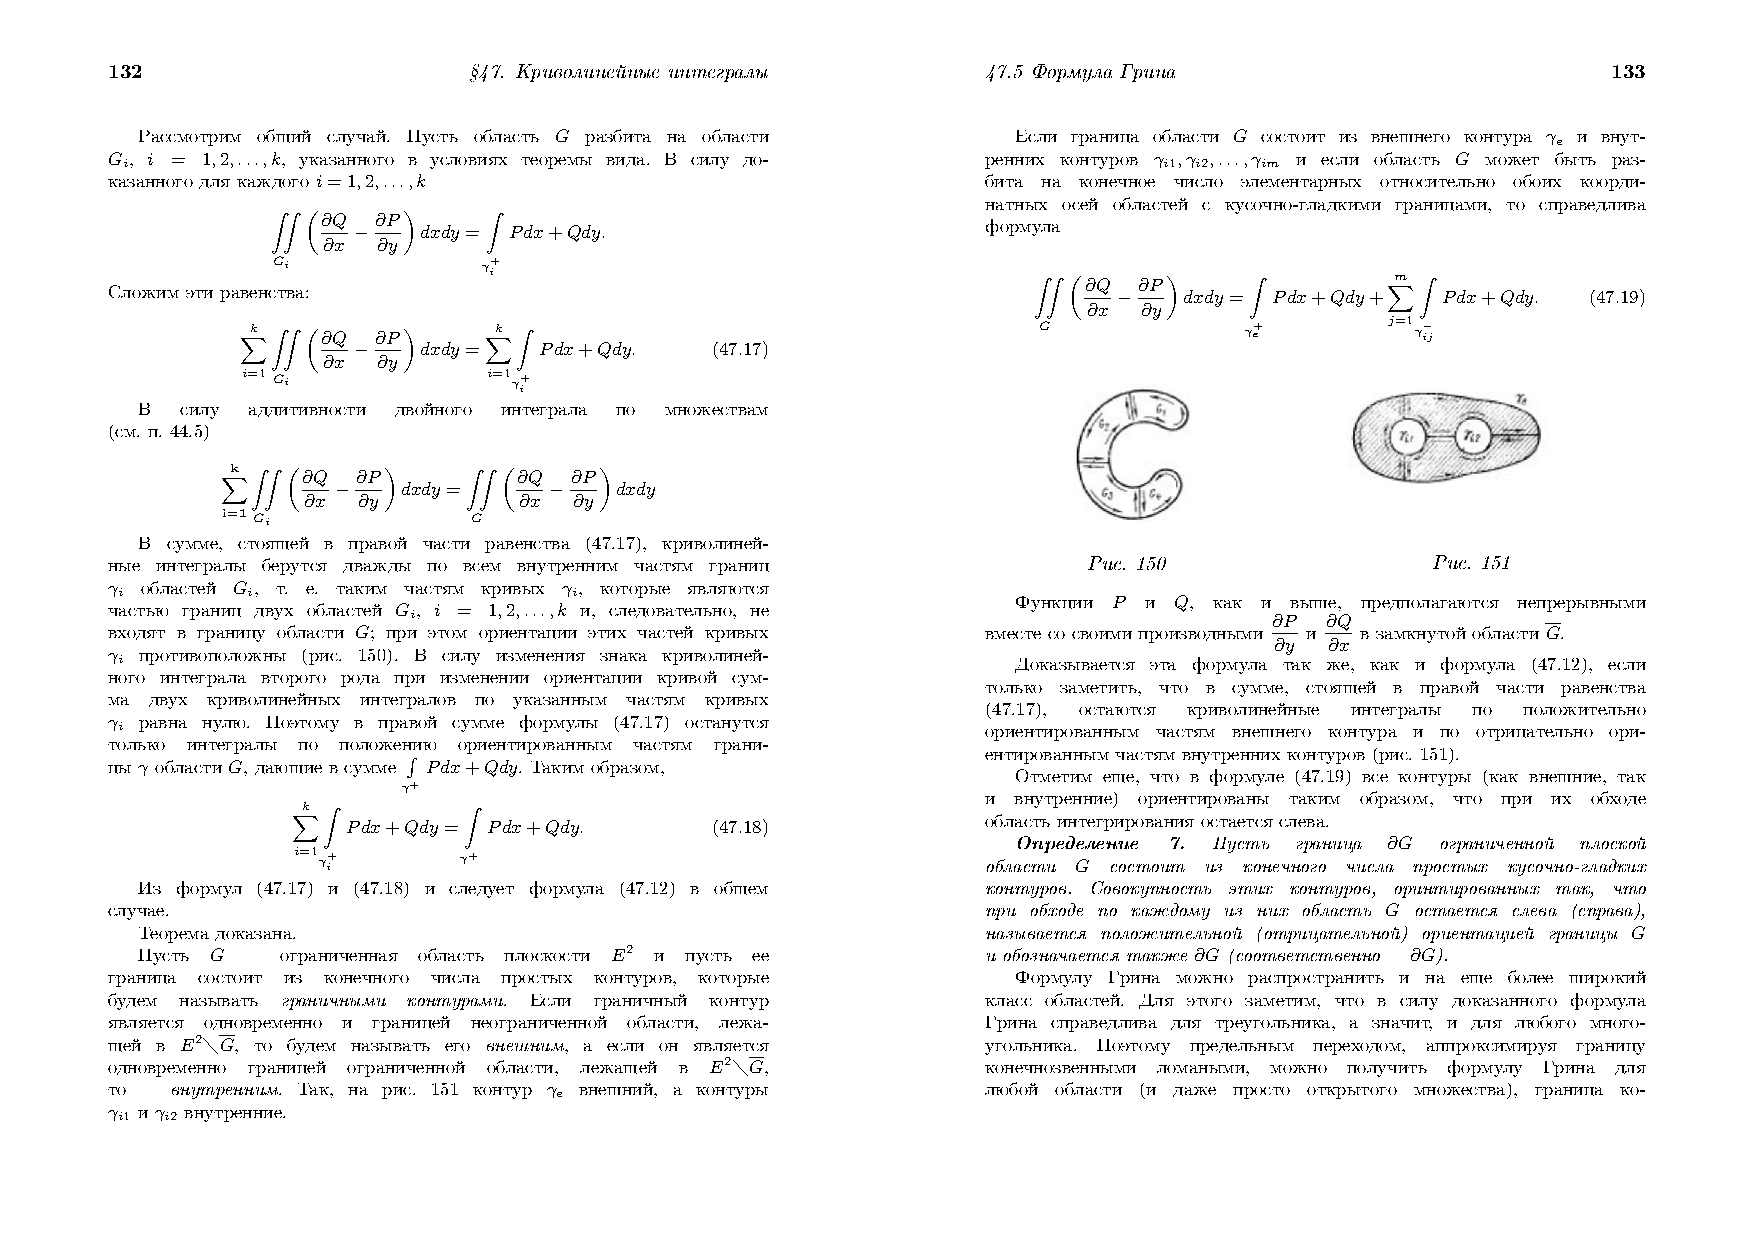
\includegraphics[scale=0.7]{1.jpg}\\
Через пару итераций был подобран $p = 25013$, удовлетворяющий условию задания.\\

Алгоритм работы: полным перебором нахожу все точки, принадлежащие кривой. Выбираю случайную точку, нахожу её порядок путём сложения самой с собой до тех пор, пока эта сумма не станет точкой $(0, 0)$. Полный перебор, как несложно догадаться, работает за $O(p^{2})$.


\subsection*{Результат работы программы}
\begin{lstlisting}
karma@mydruzhok:~/mai_study/Crypto/lab4$ python main.py 
y^2 == x^3 + 12713 * x + 7802 (mod 25013)
Order curve = 24775
Order point (18056, 24333): 37310
Time: 658.338742017746 sec.
\end{lstlisting}

\subsection*{Выводы}
Для ускорения решения задачи полного перебора используются, например, алгоритм Шуфа, использующий теорему Хассе. Его сложность $O(\log^{8}q)$, где $q$ -- число элементов поля. Еще существует метод комплексного умножения, который позволяет более эффективно находить кривые с заданным количеством точек. Однако в отличие от алгоритма Шуфа, который является универсальным, метод комплексного умножения работает только при выполнении определенных условий. 

\subsection*{Листинг программного кода}
\begin{lstlisting}[language=Python]
import time
import random


A = 1860348749492490789823288813930625381760
B = 2001637506671384833171818673149062805974


def elliptic_curve(x, y, p):
    return (y ** 2) % p == (x ** 3 + (A % p) * x + (B % p)) % p


def print_curve(p):
    print("y^2 = x^3 + {0} * x + {1} (mod {2})".format(A % p, B % p, p))


def extended_euclidean_algorithm(a, b):
    s, old_s = 0, 1
    t, old_t = 1, 0
    r, old_r = b, a

    while r != 0:
        quotient = old_r // r
        old_r, r = r, old_r - quotient * r
        old_s, s = s, old_s - quotient * s
        old_t, t = t, old_t - quotient * t

    return old_r, old_s, old_t


def inverse_of(n, p):
    gcd, x, y = extended_euclidean_algorithm(n, p)
    assert (n * x + p * y) % p == gcd

    if gcd != 1:
        raise ValueError(
            '{} has no multiplicative inverse '
            'modulo {}'.format(n, p))
    else:
        return x % p


def add_points(p1, p2, p):
    if p1 == (0, 0):
        return p2
    elif p2 == (0, 0):
        return p1
    elif p1[0] == p2[0] and p1[1] != p2[1]:
        return (0, 0)

    if p1 == p2:
        s = ((3 * p1[0] ** 2 + (A % p)) * inverse_of(2 * p1[1], p)) % p
    else:
        s = ((p1[1] - p2[1]) * inverse_of(p1[0] - p2[0], p)) % p
    x = (s ** 2 - 2 * p1[0]) % p
    y = (p1[1] + s * (x - p1[0])) % p
    return (x, -y % p)


def order_point(point, p):
    i = 1
    check = add_points(point, point, p)
    while check != (0, 0):
        check = add_points(check, point, p)
        i += 1
    return i


if __name__ == '__main__':
    p = 25013

    print_curve(p)
    points = []
    start = time.time()
    for x in range(0, p):
        for y in range(0, p):
            if elliptic_curve(x, y, p):
                points.append((x, y))

    cnt_points = len(points)
    print("Order curve = {0}".format(cnt_points))
    point = random.choice(points)

    print("Order point {0}: {1}".format(point, order_point(point, p)))
    print("Time: {} sec.".format(time.time() - start))

\end{lstlisting}

\end{document}
